\documentclass[13pt, aspectratio=169]{beamer}
\usepackage[utf8]{inputenc}
\usetheme{SimplePlus}
\usecolortheme{default}
\setbeamertemplate{navigation symbols}{}
\setbeamertemplate{headline}{}
\usepackage[brazil]{babel}
\usepackage{booktabs}
\usepackage{amsfonts,amsthm,amsmath}
\usepackage{array}
\usepackage{tabularx}
\usepackage{makecell}


\usepackage{listings}
\usepackage{verbatim}
%biblatex
\usepackage{csquotes} 
\usepackage{xpatch}

\usepackage{caption}[numbered]
\usepackage[labelformat=simple]{subcaption}
\setbeamertemplate{caption}[numbered]

\definecolor{myblue}{RGB}{31, 119, 180}
% #1f77b4 
\definecolor{myred}{RGB}{197, 0, 42}
% #c50030

\DeclareMathOperator{\EX}{\mathbb{E}}% expected value

\AtBeginSection[]
{
    \begin{frame}{Sumário}
    \tableofcontents[sectionstyle=show,
    subsectionstyle=show/shaded/hide,
    subsubsectionstyle=show/shaded/hide,
    currentsection]
  \end{frame}
}

\title{Skew t type 4 distribution -- ST4}
\author{Moisés Sales}
\date{Sep 2025}

\begin{document}
\maketitle
\section{Introdução}

\section{Definição e Propriedades}

\subsection{Função Densidade de Probabilidade e Suporte}

\begin{frame}
    \frametitle{Função Densidade de Probabilidade}
    Se $Y \sim ST4(\mu, \sigma, \nu, \tau)$, então sua função densidade de probabilidade é dada por

    \begin{equation*}
        f_Y(y | \mu, \sigma, \nu, \tau) =
            \begin{cases}
                \frac{c}{\sigma} \left[ 1 + \frac{z^2}{\nu} \right]^{-(\nu + 1)/2} \quad \text{se} \quad y < \mu \\
                \frac{c}{\sigma} \left[ 1 + \frac{z^2}{\tau} \right]^{-(\tau + 1)/2} \quad \text{se} \quad y \geq \mu \\
            \end{cases}
    \end{equation*}
    \pause
    \qquad em que
    \begin{align*}
        Z &= \frac{Y - \mu}{\sigma}, \\
        c = 2 [\sqrt{\nu} B(1/2, &\nu/2) + \sqrt{\tau} B(1/2, \tau/2)]^{-1}.
    \end{align*}
\end{frame}

\begin{frame}
    \frametitle{Suporte}
    
    \begingroup
    \setlength{\tabcolsep}{12pt}
    \renewcommand{\arraystretch}{1.9}

    \begin{table}[!ht]
        \centering    
        \begin{tabular}{l c c}
            \multicolumn{3}{c}{Intervalos} \\
            \hline
            $Y$ & $- \infty < y < \infty$ &\\
            $\mu$ & $- \infty < \mu < \infty$ & \makecell{\scriptsize moda, parâmetro de \\ \scriptsize mudança de locação}\\
            $\sigma$ & $0 < \sigma < \infty$ & \scriptsize parâmetro de escala\\
            $\nu$ & $0 < \nu < \infty$ & \makecell{\scriptsize parâmetro de peso \\ \scriptsize da cauda esquerda} \\
            $\tau$ & $0 < \tau < \infty$ & \makecell{\scriptsize parâmetro de peso \\ \scriptsize da cauda direita} \\
        \hline
        \end{tabular}
        \caption{Suporte da variável $Y$ e dos parâmetros da distribuição ST4.}    
    \end{table}

    \endgroup
\end{frame}

\subsection{Medidas da Distribuição}
\begin{frame}
    \frametitle{Medidas da Distribuição}
    \begin{itemize}
        \item Média:
            \begin{equation*}
                \EX(Y) = \mu + \sigma \EX(Z) = \mu + \sigma c \left[ \frac{\tau}{(\tau - 1} - \frac{\nu}{(\nu - 1)} \right]
            \end{equation*}
            para $\nu > 1$ e $\tau > 1$.
        \pause
        \item Mediana: 
            \begin{equation*}
                \begin{cases}
                    \mu + \sigma t \frac{(1 + k)}{4}\nu \qquad &k \leq 1 \\
                    \mu + \sigma t \frac{(3k - 1)}{4k} \tau \qquad &k > 1
                \end{cases}
            \end{equation*}
        \pause
            em que
            \begin{equation*}
                k = \frac{\sqrt{\tau} B(1/2, \tau/2)}{\sqrt{\nu} B(1/2, \nu/2)}.
            \end{equation*}
    \end{itemize}
\end{frame}

\begin{frame}
    \frametitle{Medidas da Distribuição}
    \begin{itemize}
        \item Moda: $\mu$
        \item Variância:
            \begin{equation*}
                \text{Var}(Y) = \sigma^2 \text{Var}(Z) = \sigma^2 \left\{\EX(Z^2) - [\EX(Z)]^2 \right\}
            \end{equation*}
            \pause
            em que \begin{equation*}
                \EX(Z^2) = \frac{c \tau^{3/2} B(1/2, \tau/2)}{2(\tau -2)} + \frac{c \nu^{3/2} B(1/2, \nu/2)}{2(\nu -2)}
            \end{equation*}
            para $\nu > 2$  e $\tau > 2$.
    \end{itemize}   
\end{frame}

\section{Visualização}
\subsection{Variando os Parâmetros}

\begin{frame}
    \frametitle{Variando $\mu$}

    \begin{figure}[!ht]
        \centering
        \begin{subfigure}[t]{0.4\textwidth}
            \centering
            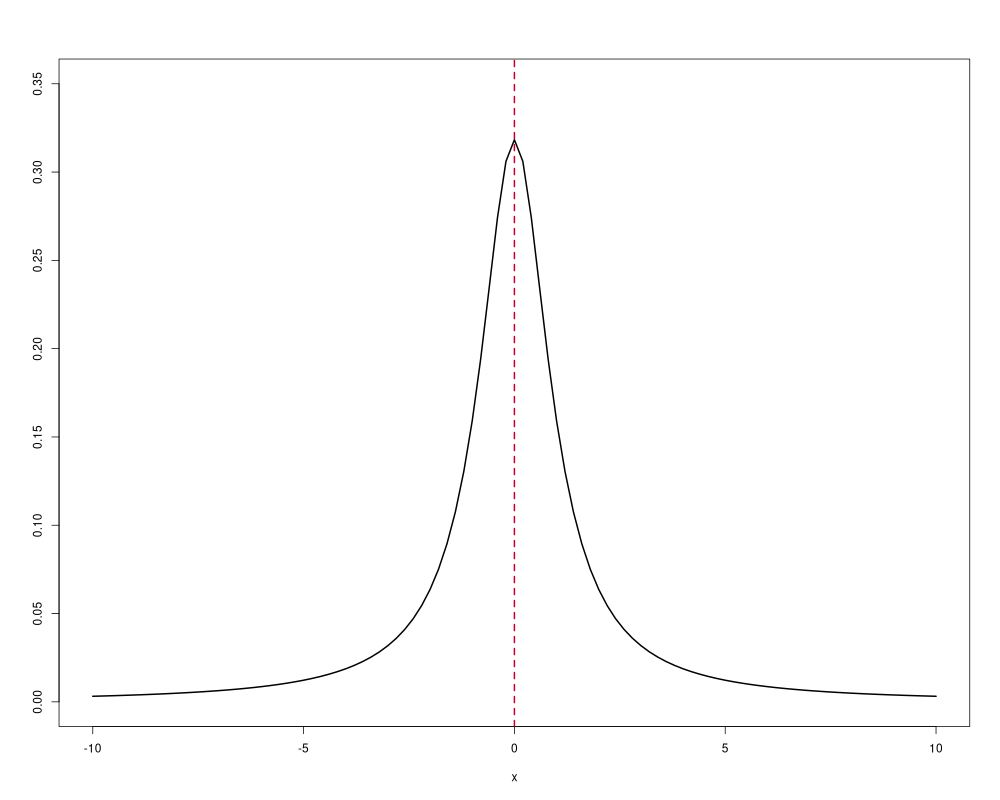
\includegraphics[width=\textwidth]{images/variando_mu_1.png}
            \caption{$\mu = 0$}
        \end{subfigure}%
        ~
        \begin{subfigure}[t]{0.4\textwidth}
            \centering
            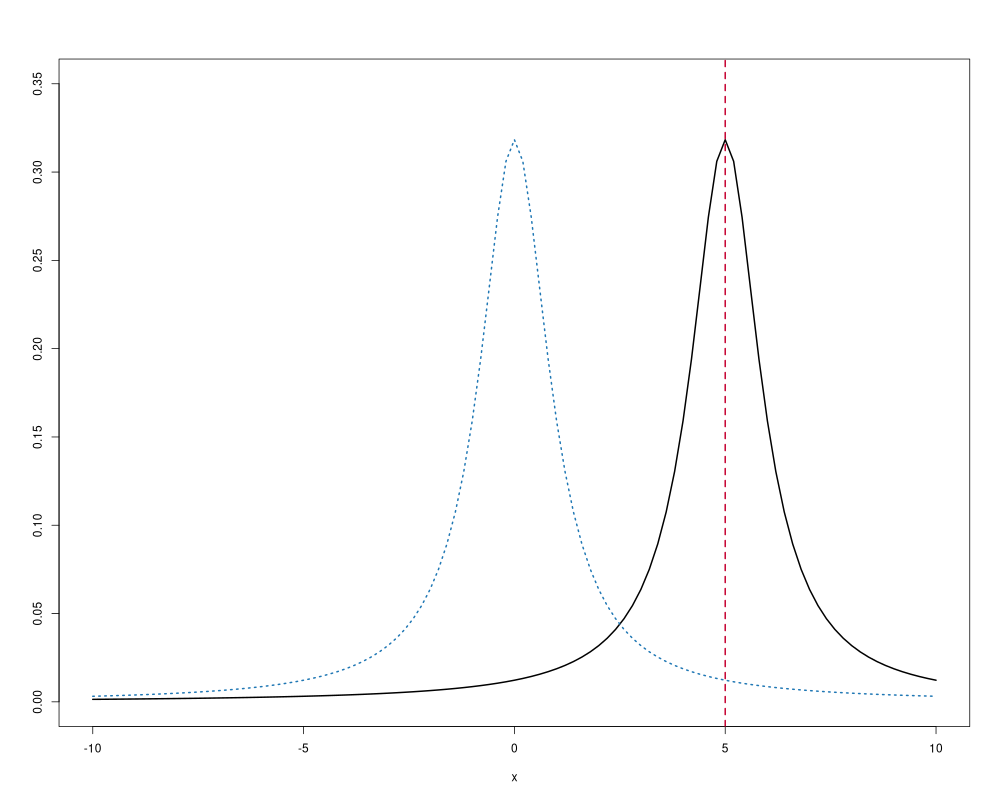
\includegraphics[width=\textwidth]{images/variando_mu_2.png}
            \caption{$\mu = 5$}
        \end{subfigure}%
        \caption{Forma da distribuição para diferentes valores de $\mu$.}
    \end{figure}

    

\end{frame}

\begin{frame}
    \frametitle{Variando $\sigma$}
    
    \begin{figure}[!ht]
        \centering
        \begin{subfigure}[t]{0.4\textwidth}
            \centering
            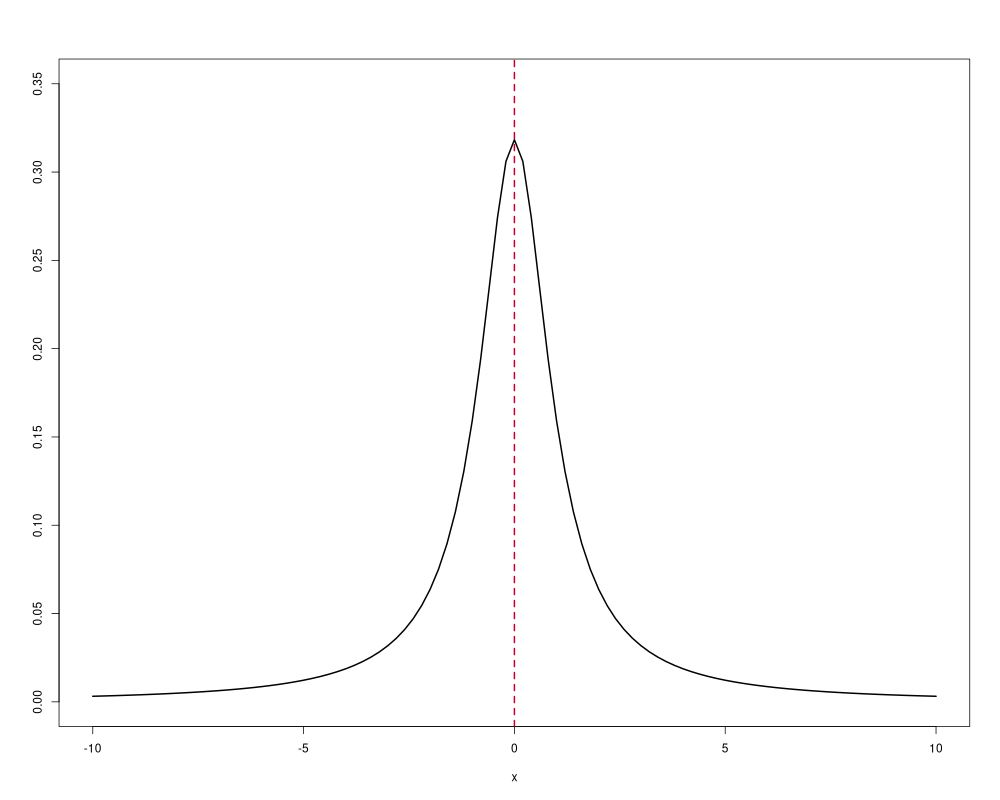
\includegraphics[width=\textwidth]{images/variando_sigma_1.png}
            \caption{$\sigma = 1$}
        \end{subfigure}%
        ~
        \begin{subfigure}[t]{0.4\textwidth}
            \centering
            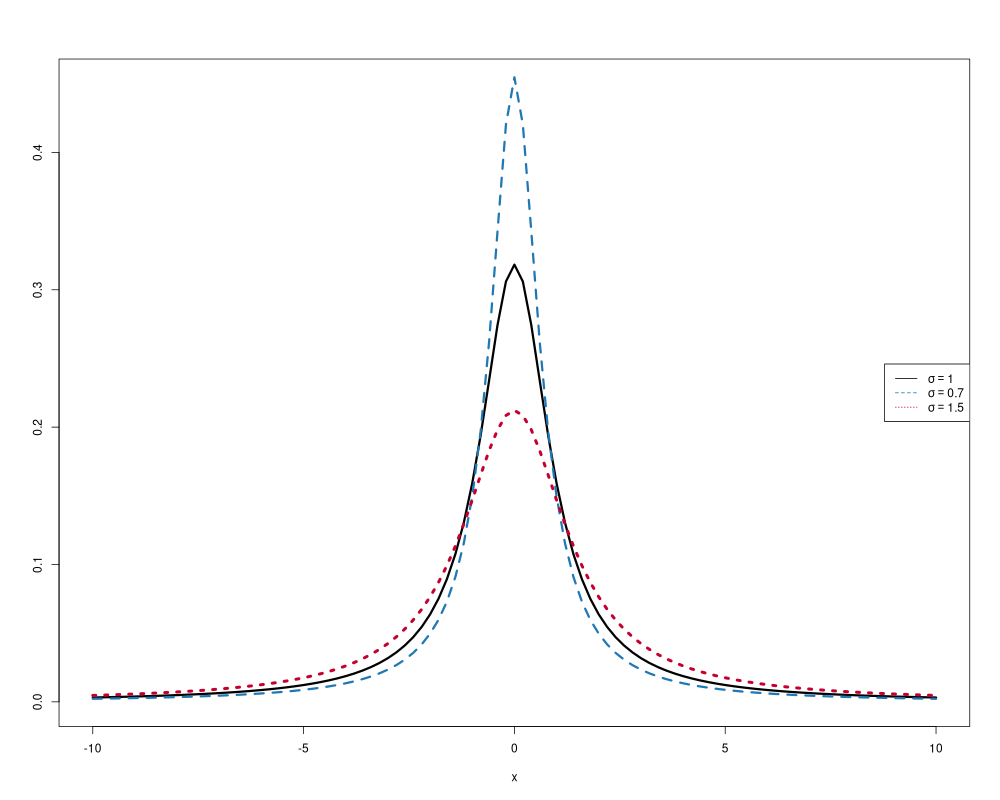
\includegraphics[width=\textwidth]{images/variando_sigma_2.png}
            \caption{$\sigma = 0.7, \,\, 1.5$}
        \end{subfigure}%
        \caption{Forma da distribuição para diferentes valores de $\sigma$.}
    \end{figure} 

\end{frame}

\begin{frame}
    \frametitle{Variando $\nu$}
    
    \begin{figure}[!ht]
        \centering
        \begin{subfigure}[t]{0.4\textwidth}
            \centering
            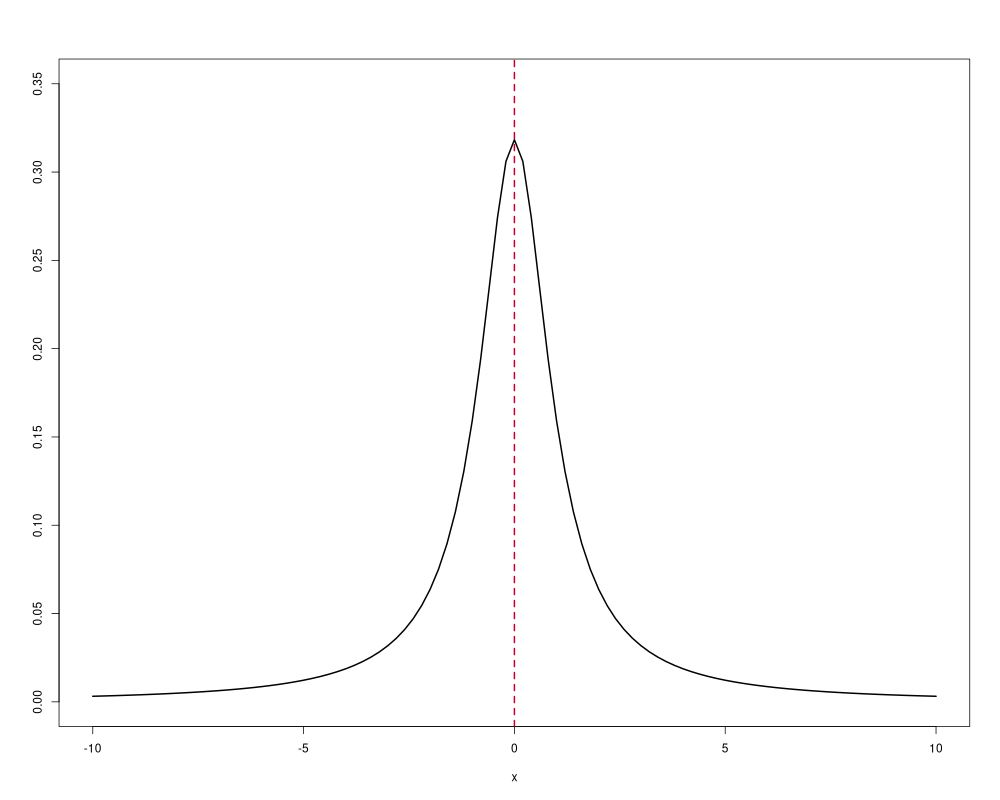
\includegraphics[width=\textwidth]{images/variando_mu_1.png}
            \caption{$\nu = 1$}
        \end{subfigure}%
        ~
        \begin{subfigure}[t]{0.4\textwidth}
            \centering
            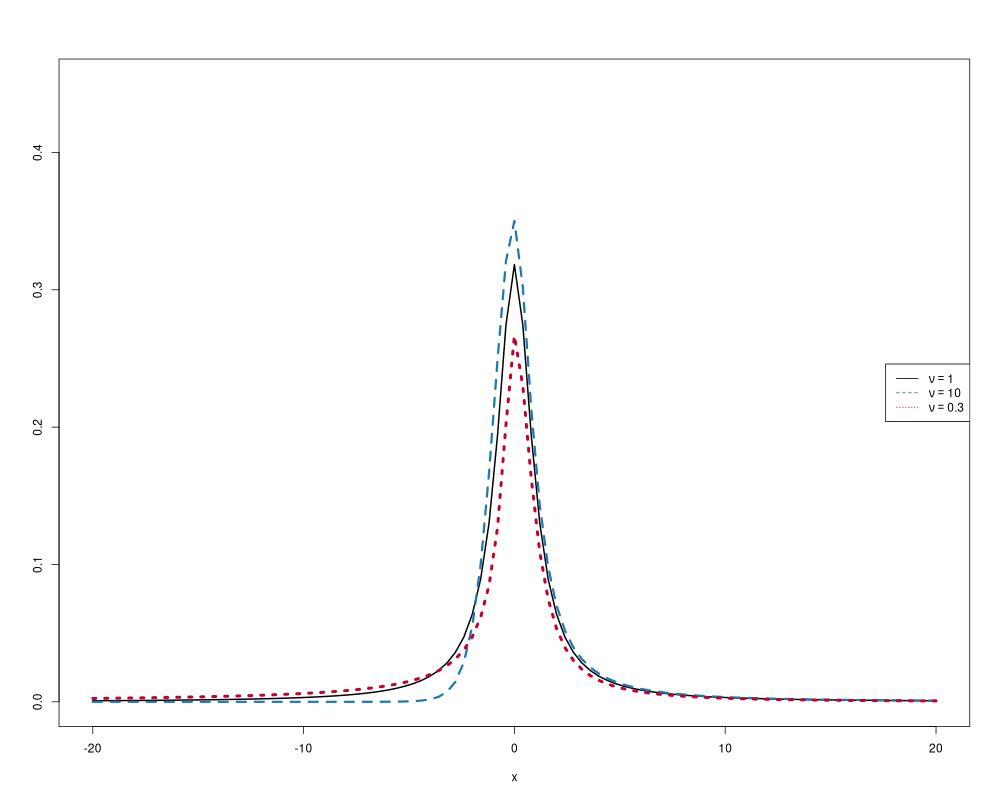
\includegraphics[width=\textwidth]{images/variando_nu_2.png}
            \caption{$\nu = 0.3, \,\, 30$}
        \end{subfigure}%
        \caption{Forma da distribuição para diferentes valores de $\nu$.}
    \end{figure} 

\end{frame}

\begin{frame}
    \frametitle{Variando $\tau$}

    \begin{figure}[!ht]
        \centering
        \begin{subfigure}[t]{0.4\textwidth}
            \centering
            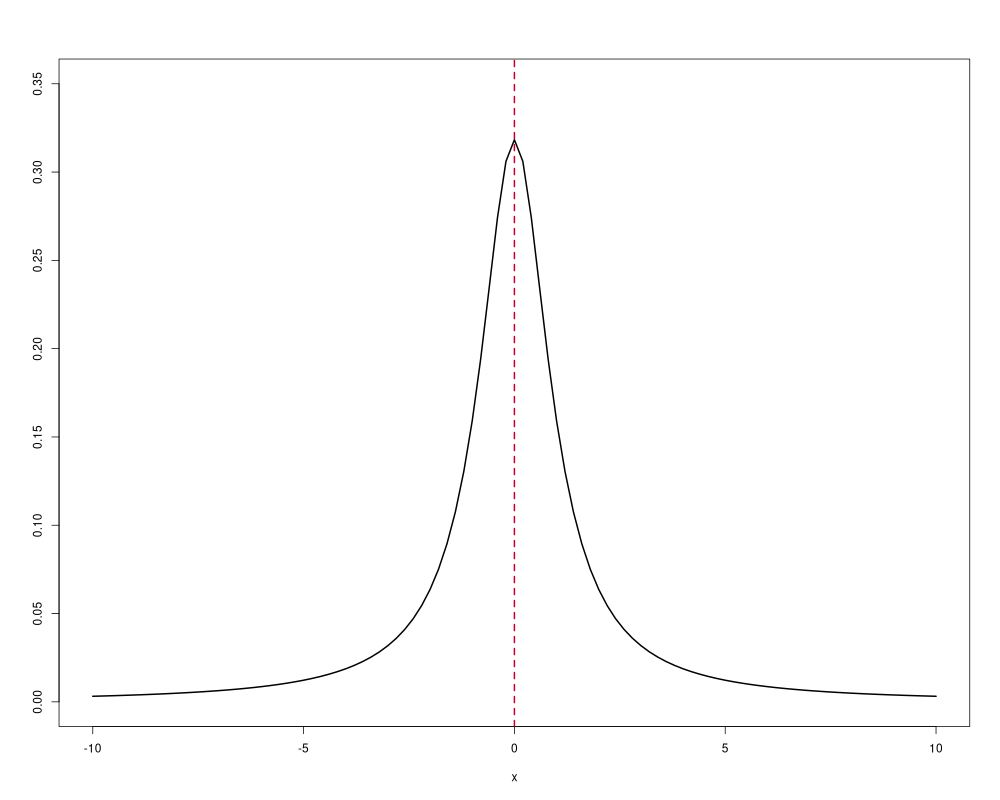
\includegraphics[width=\textwidth]{images/variando_mu_1.png}
            \caption{$\tau = 1$}
        \end{subfigure}%
        ~
        \begin{subfigure}[t]{0.4\textwidth}
            \centering
            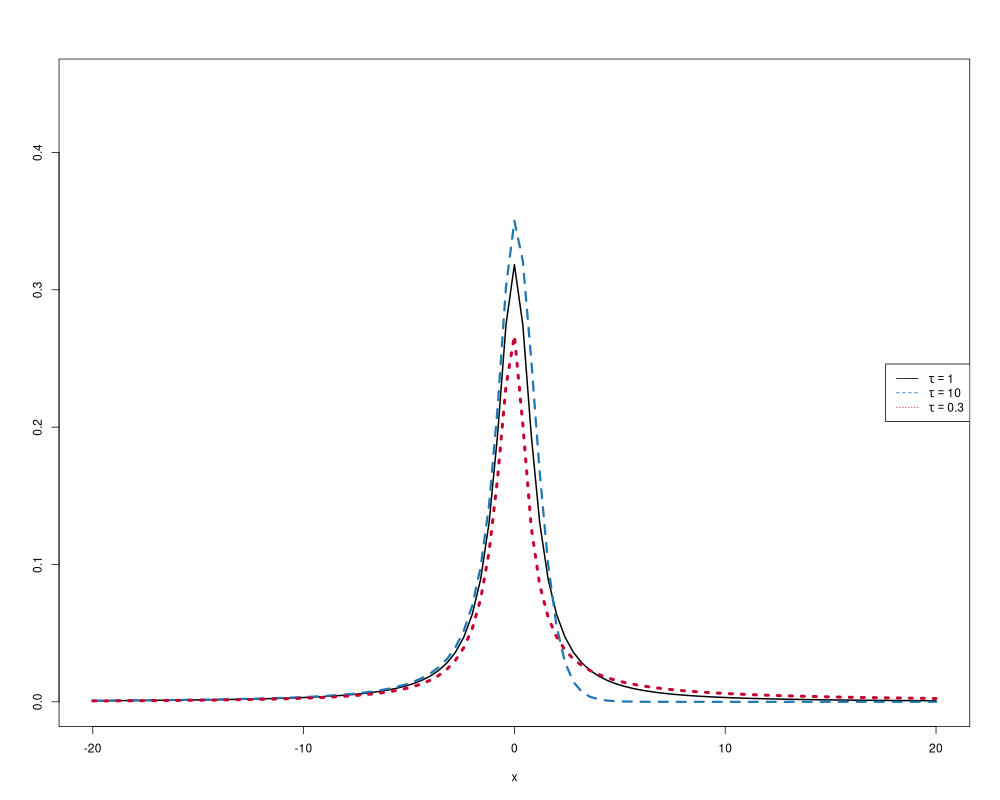
\includegraphics[width=\textwidth]{images/variando_tau_2.png}
            \caption{$\tau = 0.1, \,\, 50$}
        \end{subfigure}%
        \caption{Forma da distribuição para diferentes valores de $\tau$.}
    \end{figure}
\end{frame}

\begin{frame}
    \frametitle{Exemplos}

    \begin{figure}[!ht]
        \centering
        \begin{subfigure}[t]{0.4\textwidth}
            \centering
            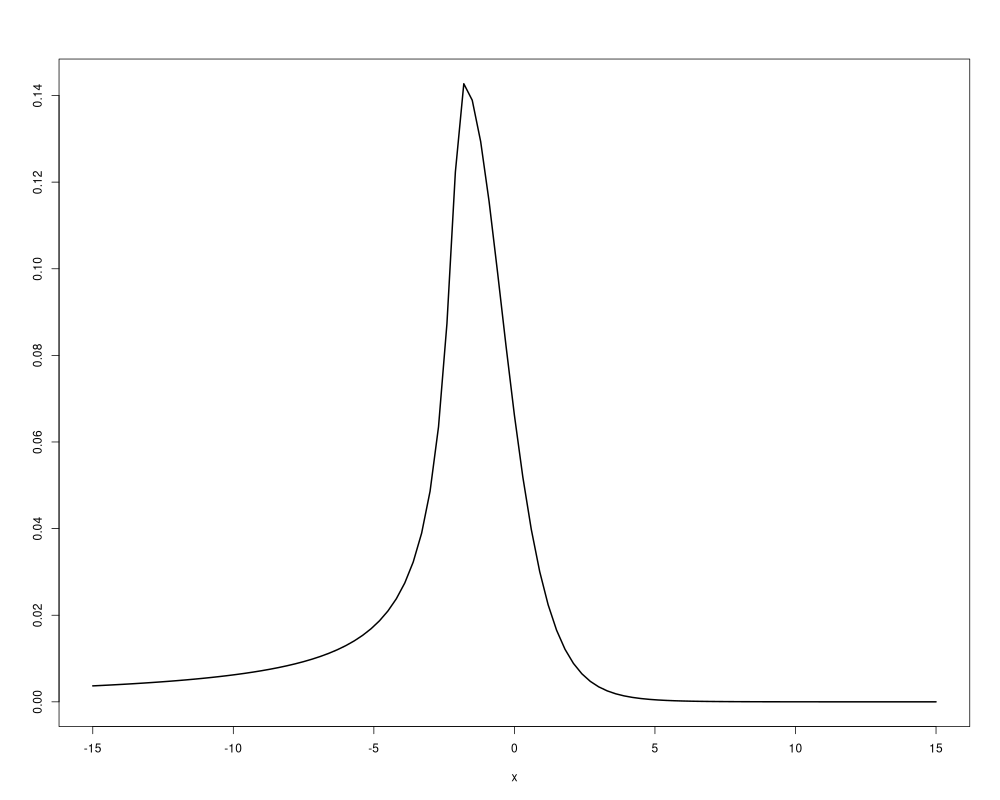
\includegraphics[width=\textwidth]{images/dist_1.png}
            \caption{$\mu = -1.83, \sigma = 1.5, \nu = 0.1, \tau = 7.8$}
        \end{subfigure}%
        ~
        \begin{subfigure}[t]{0.4\textwidth}
            \centering
            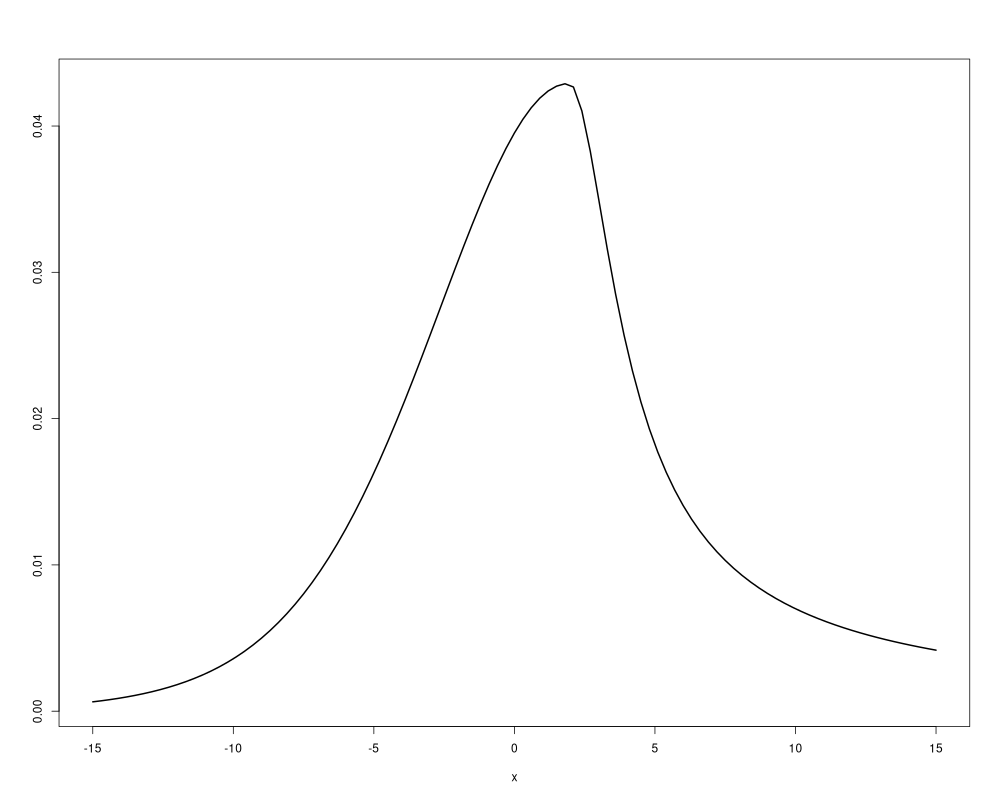
\includegraphics[width=\textwidth]{images/dist_2.png}
            \caption{$\mu = 1.94, \sigma = 5, \nu = 10, \tau = 0.1$}
        \end{subfigure}%
        \caption{Formas da distribuição para diferentes valores dos parâmetros.}
    \end{figure}
\end{frame}

\section{Exemplo Prático}

\section{Conclusão}



\end{document}
